\section{Durchführung}
\label{sec:Durchführung}

Um Messungen mit dem Geiger-Müller-Zählrohr durchzuführen wird der Versuch wie in \autoref{fig:aufbau} aufgebaut.
\begin{figure}[H]
    \centering
    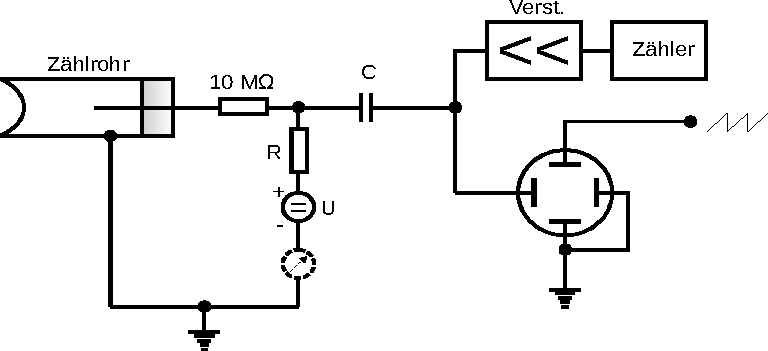
\includegraphics{Abbildungen/Abb_5.pdf}
    \caption {Schaltkreis des Versuchs.\cite{V703}}
    \label{fig:aufbau}
\end{figure}
Die Funktion des Geiger-Müller-Zählrohrs wird in \autoref{sec:Theorie} bereits erläutert.
Das Geiger-Müller-Zählrohr ist an eine Spannungsquelle angeschlossen. Zudem kann über ein Amperemessgerät am Zählrohr der
Zählrohrstrom $I$ abgelesen werden.
Außerdem ist es über einen Verstärker an einen Zähler gekoppelt.


\subsection{Charakteristik des Zählrohrs}
\label{sub:charakteristik_durch}

Um die Charakteristik des Zählrohrs aufzunehmen wird vor das Zählrohrfenster eine $\beta$-Quelle positioniert.
In Abhängigkeit von der Spannung wird die Zählrate gemessen.
Die Messung der Zählrate wird für Spannungen im Abstand von $\qty{10}{\volt}$ in einem Bereich von $\qty{320}{\volt}$ bis $\qty{700}{\volt}$ 
für jeweils $t=\qty{60}{\second}$ durchgeführt, damit die Standardabweichung der Poissonverteilung unter $\qty{1}{\percent}$ bleibt.

Zudem wird für die spätere Bestimmung der freigesetzten Ladungen pro Teilchen der Zählrohrstrom aufgenommen.
Damit Dauerentladungen verhindert werden, die das Zählrohr zerstören können, wird die Spannung nicht über $\qty{700}{\volt}$ erhöht.


\subsection{Totzeit des Zählrohrs}
\label{sub:totzeit_durch}

Die Totzeit des Zählrohrs kann mit zwei verschiedenen Methoden bestimmt werden.

Zunächst wird der Ausgang des Zählrohrs an das Oszilloskop angeschlossen.
Auf dem Bildschirm ist dann eine Kurve zu sehen, woraus die Totzeit mithilfe der Skala abgelesen wird.

Zudem wird die Totzeit mit der Zwei-Quellen-Methode bestimmt.
Hierfür wird zuerst die Zählrate $N_1$ des einen Präparats gemessen.
Dann wird eine zweite Quelle hinzugefügt und die Zählrate $N_{12}$ wird bestimmt.
Zuletzt wird noch der Wert für $N_2$ gemessen und die Totzeit errechnet.






